\documentclass[aspectratio=169]{beamer}  % 16:9 aspect ratio

% Use a clean theme as base
\usetheme{default}
\usecolortheme{default}

% Custom colors from HKUST logo
\definecolor{hkustblue}{RGB}{0, 51, 119}    % Navy blue from logo
\definecolor{hkustgold}{RGB}{180, 141, 61}  % Golden brown from logo
\definecolor{lightgray}{RGB}{236, 240, 241}

% Customize the appearance
\setbeamercolor{structure}{fg=hkustblue}
\setbeamercolor{background canvas}{bg=white}
\setbeamercolor{normal text}{fg=hkustblue}
\setbeamercolor{frametitle}{fg=hkustblue,bg=white}
\setbeamercolor{itemize item}{fg=hkustgold}
\setbeamercolor{itemize subitem}{fg=hkustgold}
\setbeamercolor{block title}{fg=white,bg=hkustblue}
\setbeamercolor{block body}{fg=hkustblue,bg=lightgray}
\setbeamercolor{title}{fg=hkustblue}
\setbeamercolor{subtitle}{fg=hkustgold}

% Remove navigation symbols
\setbeamertemplate{navigation symbols}{}

% Customize frame title
\setbeamertemplate{frametitle}{
    \vspace*{0.5cm}
    \insertframetitle
    \vspace*{0.2cm}
    \begin{beamercolorbox}[wd=\paperwidth,ht=0.2pt]{structure}
    \end{beamercolorbox}
}

% Customize itemize bullets
\setbeamertemplate{itemize item}{\small\raise0.5pt\hbox{\textbullet}}
\setbeamertemplate{itemize subitem}{\tiny\raise1.5pt\hbox{\textbullet}}

% Packages
\usepackage{graphicx}
\usepackage{amsmath}
\usepackage{hyperref}

% Title page information
\title{Moment Inequality and Partial Identification in Industrial Organization}
\subtitle{Handbook of IO, Volume 4, Chapter 5}
\author{Presented by: Hang XU, Xinrui LIU}
\institute{Hong Kong University of Science and Technology}
\date{\today}

\begin{document}

% Title page
\begin{frame}
    \titlepage
\end{frame}

% Table of contents
% \begin{frame}{Outline}
%     \tableofcontents
% \end{frame}

% Get a intro page of each section
\AtBeginSection[]
{
    \begin{frame}
        \frametitle{Outline}
        \tableofcontents[currentsection]
    \end{frame}
}

% Mark the page number on a specific position
\addtobeamertemplate{navigation symbols}{}{%
    \usebeamerfont{footline}%
    \usebeamercolor[fg]{footline}%
    \hspace{1em}%
    \insertframenumber/\inserttotalframenumber
}


% Section 1
\section{Introduction}
\begin{frame}{Point Identification}
    \begin{block}{Point Identification}
        Estimating model parameters as a single value, e.g., $\hat{\theta} = 0.5$.
    \end{block}
    \pause
    \begin{itemize}
        \item In traditional econometrics, we often try to find point identification \textbf{with a cost} of adding more assumptions (to improve identifying power).
        \item Common assumptions include: Certain distributions of error terms (e.g., logit model); Independence of error terms.
        \item If assumptions are satisfied, one can always obtain the true value of the parameter by using an infinite amount of data.
        \item But in reality, these assumptions are often violated or not well justified by economic theory (e.g., correlation between error terms and regressor).
        \item \textbf{Problem}: Two researchers using the same data may reach different conclusions due to different assumptions.
    \end{itemize}
\end{frame}

\begin{frame}{Partial Identification}

    \begin{itemize}
        \item Need to find out what can be learned from the data \textbf{without imposing strong assumptions} -- May give up point identification and turn to partial identification.
        \pause
        \begin{block}{Partial Identification}
            Estimating model parameters as a set, e.g., $\hat{\theta} \in [0.3, 0.7]$.
        \end{block}
        \pause
        \item Cannot know the true value of the parameter even with an infinite dataset, but can still reveal some insights about the object of interest.
        \item Usually, the partial identification of the parameter is derived from a set of inequalities, which are called \textbf{moment inequalities}.
        \item The inequalities are derived from optimizing behavior based on economic theory (e.g., revealed preferences) or simply the statistical properties from the data.

    \end{itemize}
\end{frame}

\begin{frame}{Roadmap}
    \begin{itemize}
        \item Partial identification is widely used in empirical IO, especially in
        \begin{itemize}
            \item Models with measurement errors or unobserved heterogeneity,
            \item Models based on revealed preference,
            \item Strategic interaction models among multiple agents (e.g., market entry, auction),
            \item Models with multiple equilibria or incomplete information.
        \end{itemize}
    \vspace{0.5cm}
        \item Partial identification also gives challenges for estimation and inference:
        \begin{itemize}
            \item Estimation: How do we estimate a set? What is a ``good" estimate of set?
            \item Inference: How to test an hypothesis about true parameters with partial identification?
        \end{itemize}
    \end{itemize}
\end{frame}

\begin{frame}{Acknowledgement}
This presentation is based on
    \begin{itemize}
        \item Chapter 5: \textit{Moment Inequality and Partial Identification in Industrial Organization} from the Handbook of Industrial Organization, Volume 4,
        \item \textit{Introduction to Partial Identification} from C. Bontemps' lecture notes.
    \end{itemize}
\end{frame}

% Section 2
\section{Example 1: Measurement Error Models}

\begin{frame}{A Warm-up: Frisch (1934): Measurement Error Models}
    \begin{itemize}
        \item \textbf{Example}: Consider a simple linear regression model $y^* = \beta x^* + u$.
        \item If we assume $E(x^* u) = 0$, we can estimate a consistent $\beta$ as $\hat{\beta} = \frac{\sum_{i=1}^n (x^*_i - \overline{x}) (y^*_i - \overline{y})}{\sum_{i=1}^n (x^{*}_{i} - \overline{x})^2}$.
        \item Now, suppose both $x^*$ and $y^*$ are measured with errors:
        \begin{align*}
        x = x^* + v_x \\
        y = y^* + v_y
        \end{align*}
        Where $v_x, v_y$ are unobserved measurement errors with i.i.d. distribution.
        \item How to estimate $\beta$ in the true model by only observing ($x, y$)?
    \end{itemize}
\end{frame}

\begin{frame}{A Warm-up: Frisch (1934): Measurement Error Models (Cont'd)}
    The true model implies
    \begin{align*}
    y = \beta x + \underbrace{u + v_y - \beta v_x }_{w}
    \end{align*}
    and if we regress $y$ on $x$:
    \begin{align*}
    \hat{\beta} = \beta + \frac{Cov(x, w)}{Var(x)}
    \end{align*}
\begin{itemize}
    \item This leads to inconsistency of the estimation. 
    \item Traditional methods (e.g., IV) can get point identification of $\beta$ if conditions hold.
    \item Alternatively, we can use partial identification to get a set of $\hat{\beta}$ by finding some moment inequalities.
\end{itemize}

\end{frame}

\begin{frame}{A Warm-up: Frisch (1934): Measurement Error Models (Cont'd)}
The model imposes some equations in second order moments of observables:
\begin{align}
    Var(x) &= Var(x^*) + Var(v_x) \\
    Var(y) &= Var(y^*) + Var(v_y) \geq \beta^2 Var(x^*) + Var(v_y) \\
    Cov(x, y) &= Cov(x^* + v_x, y^* + v_y)= \beta Var(x^*) \\
    (2) + (3) \rightarrow Var(y) &\geq \beta Cov(x, y) + Var(v_y)
\end{align}

Two inequalities can be derived based on the statistical properties of variance:
\begin{itemize}
    \item $Var(v_x) \geq 0$ $\rightarrow$ $\beta \geq \frac{Cov(x, y)}{Var(x)}$
    
    \item $Var(v_y) \geq 0$ $\rightarrow$ $\beta \leq \frac{Var(y)}{Cov(x, y)}$
    \item Then, we can get a set of $\hat{\beta} \in [\frac{Cov(x, y)}{Var(x)}, \frac{Var(y)}{Cov(x, y)}]$
\end{itemize}
\end{frame}


% Section 3
\section{Example 2: Models Based on Revealed Preference}
\begin{frame}{Revealed Preference}
    \begin{itemize}
        \item Revealed preference theory is a method to infer consumer preferences from observed choices.
        \item The theory is based on the assumption that consumers' choices are consistent with their preferences.
        \item The theory can be used to derive moment inequalities for partial identification.
        \item Formally, let $\pi(d_i, d_{-i}, y_i, \theta)$ be the pay-off agent $i$ receives from choosing action $d_i$ given its competitors chose $d_{-i}$ and other determinants $y_i$, we have:
        \begin{align*}
            E\left[\pi(d_i, d_{-i}, y_i, \theta) | I_i\right] \geq E\left[\pi(d, d_{-i}, y_i, \theta) | I_i\right] \quad \forall d \in \mathbb{D}_i
        \end{align*}
        Where $I_i$ is the information set, and $\mathbb{D}_i$ is the choice set available to agent $i$.
        \item The expectation is taken since competitors actions or other determinants might be random at the time of decision.
    \end{itemize}

\end{frame}

\begin{frame}{Katz (2007): Shoppers Driving Time Costs}
    \begin{itemize}
        \item Katz (2007) studies the costs shoppers assign to driving to a supermarket, which is important for zoning laws and public transportation policy.
\vspace{0.5cm}
        \item This problem involves a two-stage decision process: agent $i$'s decision $d_i = (s_i, b_i)$,
            \begin{itemize}
                \item First, choose a supermarket (store) $s_i$.
                \item Then, choose products to purchase (a complex choice set of possible bundles), say the basket $b_i$.
            \end{itemize}
        \end{itemize}

\end{frame}


\begin{frame}{Katz (2007): Shoppers Driving Time Costs (Cont'd)}
    \begin{itemize}
    \item The utility functions of the agent with $z_i$ characteristics are additively separable functions of:
            \begin{itemize}
                \item The utility of the basket bought $u\left(b_i, z_i\right)$,
                \item The expenditure on the basket $e\left(b_i, s_i\right)$,
                \item Driving time to the store $\theta_i dt\left(s_i, z_i\right)$.
            \end{itemize}
            \vspace{0.5cm}
            Utility function is:
        \begin{align*}
            \pi(d_i, z_i, \theta) = u(b_i, z_i) - e(b_i, s_i) - \theta_i dt(s_i, z_i)
        \end{align*}
        Where $\theta_i = \theta_0 + v_i$ is the parameter of interest (the dollar value of driving time), and $v_i$ is the unobserved preference for driving time.
        \end{itemize}

\end{frame}

\begin{frame}{Katz (2007): Shoppers Driving Time Costs (Cont'd)}
    \begin{itemize}
    \item By using revealed preference, we compare the actual choice, $d_i$, to the alternative $d_{i}^{f}$ of purchasing:

        \begin{itemize}
            \item The \textcolor{red}{same} basket $b_i$ of goods,
            \item At a store $s_i^{f}$ that is \textcolor{red}{farther away} from the agent's home than the actual store $s_i$.
        \end{itemize}
    Thus, we have:
    \begin{align*}
        \Delta \pi(d_i, d_i^f, z_i, \theta) &= \pi(d_i, z_i, \theta) - \pi(d_{i}^{f}, z_i, \theta) \\
        &= - \Delta e(b_i, s_i, s_i^f) - (\theta_0 + v_i) \Delta dt(s_i, s_i^f, z_i) \geq 0
    \end{align*}
    \item Notice that choosing a different basket at $d_{i}^{f}$ just reinforces the inequality.
    \item Then we have:
    \begin{align*}
        \theta_0 + v_i \quad \textcolor{red}{\geq} \quad - \frac{\Delta e(b_i, s_i, s_i^f)}{\textcolor{red}{\Delta dt}(s_i, s_i^f, z_i)}
    \end{align*}
    \end{itemize}

\end{frame}


\begin{frame}{Katz (2007): Shoppers Driving Time Costs (Cont'd)}
    \begin{itemize}
    \item Assume that $v_i$ follows a distribution with mean zero: $E(v_i) = 0$.
    \item Then we can get the moment inequality by aggregating over all agents:
    \begin{align*}
        \theta_0 \geq - \frac{E[\Delta e(b_i, s_i, s_i^f)]}{E[\Delta dt(s_i, s_i^f, z_i)]}
    \end{align*}
    \item Similar approach can be applied to a store that is \textcolor{red}{closer} to the agent's home: $s_i^{c}$.
    \begin{align*}
        \theta_0 \leq - \frac{E[\Delta e(b_i, s_i, s_i^c)]}{E[\Delta dt(s_i, s_i^c, z_i)]}
    \end{align*}
    \item This approach \textcolor{red}{eliminates} the needs to specify: 
        \begin{itemize}
            \item The specific distribution assumption of $v_i$ (where MNL model is often used),
            \item The choice set of the basket $b_i$ and store $s_i$ for each agent,
            \item The two-stage decision problem.
        \end{itemize} 
    \end{itemize}
\end{frame}

% Section 4
\section{Examples with Partial Identification: Strategic Interactions}

\begin{frame}{Strategic Interactions}
    \begin{itemize}
        \item The previous case is a \textcolor{red}{single-agent model}, where the agent's decision depends on the agent's own characteristics.
        \item In many IO models, agents' decisions depend on the decisions of others, which is called strategic interactions, or \textcolor{red}{multi-agent models}.
        \item The payoffs in multi-agent models are often functions of actions of all agents, and the agents' actions are interdependent.
        \item Models with strategic interactions may have multiple equilibria, incomplete information, or other complications where MNL with MLE are not applicable.
        \item In such models, the revealed preference approach tends to use only a subset of conditions implied by the model, thereby leading to learning less about the parameters (may have a wide set of estimates).
        \item Thus, other conditions (e.g., equilibrium conditions, equilibria selections, etc.) are needed to narrow down the set of estimates.
    \end{itemize}
\end{frame}

\begin{frame}{A Market Entry Game with Complete Information}
\begin{itemize}
    \item Two firms $i = 1, 2$ decide whether to enter a market: $d_i = {1,0}$ with $0$ to be not. The payoff of firm $i$ is:
    \begin{align*}
        \pi_1 = d_1 \times (x_1 \beta_1 + \Delta_1 d_2 + \epsilon_1) \\
        \pi_2 = d_2 \times (x_2 \beta_2 + \Delta_2 d_1 + \epsilon_2)
    \end{align*}

\begin{figure}
    \centering
    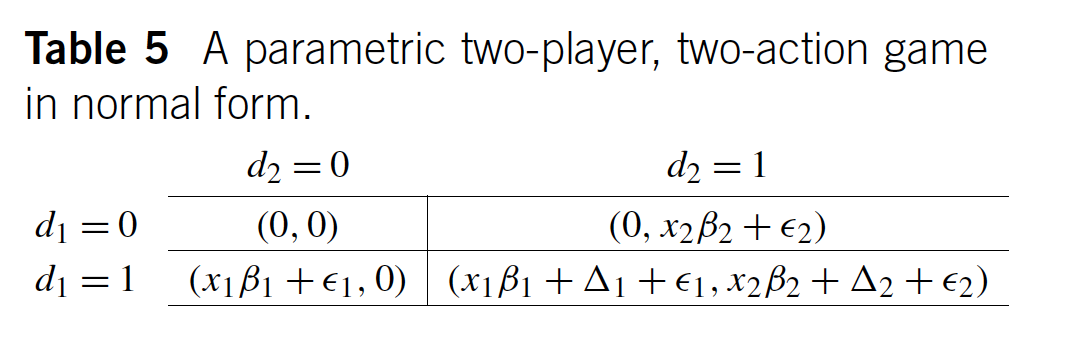
\includegraphics[width=0.6\textwidth]{market entry game table.png}
\end{figure}

    \item Firms have complete information about the other firm's profit function,
    \item Assume both $\Delta_1$ and $\Delta_2$ are negative, a competition effect,
    \item Only focus on pure strategy Nash equilibrium.
    \end{itemize}
\end{frame}

\begin{frame}{A Market Entry Game with Complete Information (Cont'd)}
Shocks $\epsilon_i \perp  x_i$ are known to the firm but not to the econometrician:
\begin{itemize}
    \item Firms observe all components of the payoff, including $\epsilon_i$, so their decisions satisfy:
    \begin{align*}
        d_i = \mathbf{1}\{\pi_i \geq 0\} \quad for \quad i = 1, 2
    \end{align*}
    \item The econometrician can only observe the entry decisions $d_i$: a pair of indicators $(d_1, d_2)$ and the characteristics $x_i$.
    \begin{itemize}
        \item If $(d_1, d_2) = (1, 0)$ is observed (firm 1 is the monopolist), $\Rightarrow$ $x_1\beta_1 + \epsilon_1 \geq 0$ and $x_2 \beta_2 + \Delta_2 + \epsilon_2 \leq 0$, $\Rightarrow$ A \textcolor{red}{necessary condition} for $(1, 0)$ to be the equilibrium;
        \item From a reverse logic, when $x_1\beta_1 + \epsilon_1 \geq 0$ and $x_2 \beta_2 + \epsilon_2 \leq 0$, $\Rightarrow$ $(1, 0)$ is a dominant strategy equilibrium, $\Rightarrow$ A \textcolor{red}{sufficient condition} for $(1, 0)$ to be the equilibrium.
    \end{itemize}
    \item The aim is to learn the vector of parameters $\theta = (\beta_1, \beta_2, \Delta_1, \Delta_2)$.

\end{itemize}
\end{frame}

\begin{frame}{A Market Entry Game with Complete Information (Cont'd)}
\begin{itemize}
    \item It seems we can obtain a point identification of $\theta$ by maximizing the likelihood function of the observed data if assuming the distributions of $\epsilon_i$.
    \item i.e., choose $\theta$ such that we match the observed four choice probabilities $p_{ij} = P(d_1 = i, d_2 = j)$ as good as possible.
    \item However, since \textcolor{red}{multiple equilibria} exists in some regions, the choice probability for some outcomes \textcolor{red}{cannot} be written as a function of $\theta$ (the pay-off functions), even with the distributional assumption of $\epsilon_i$:
    \begin{itemize}    
        \item Within certain range of $\epsilon$, the outcome is still random since which equilibrium is selected is random.
    \end{itemize}
\end{itemize}
\end{frame}

\begin{frame}{A Market Entry Game with Complete Information (Cont'd)}
\begin{itemize}
    \item Specify the choice probabilities as (assuming $\Delta_1$ and $\Delta_2$ are negative):
\begin{align*}
    p_{00} = P(d_1 = 0, d_2 = 0 | x) &= P \left(\epsilon_1 \leq -x_1 \beta_1, \epsilon_2 \leq -x_2 \beta_2\right) \\
    p_{11} = P(d_1 = 1, d_2 = 1 | x) &= P \left(\epsilon_1 \geq -x_1 \beta_1 - \Delta_1, \epsilon_2 \geq -x_2 \beta_2 - \Delta_2\right) \\
    p_{10} = P(d_1 = 1, d_2 = 0 | x) &= P \left(\epsilon_1 \geq -x_1 \beta_1, \epsilon_2 \leq -x_2 \beta_2 - \Delta_2, \epsilon \notin S_\beta \right) \\
    &+ \textcolor{red}{P \left(d_1 = 1, d_2 =0 | x, \epsilon \in S_\beta \right)} \times P\left(\epsilon \in S_\beta\right) \\
    p_{01} = P(d_1 = 0, d_2 = 1 | x) &= 1 - p_{00} - p_{11} - p_{10}
\end{align*}
\item Where $S_\beta = \left\{\epsilon: -x_1 \beta_1 \leq \epsilon_1 \leq -x_1 \beta_1 - \Delta_1, -x_2 \beta_2 \leq \epsilon_2 \leq -x_2 \beta_2 - \Delta_2\right\}$ are the regions where the equilibrium is not unique: $(1, 0)$ and $(0, 1)$ are both equilibria.
\item For $p_{00}$ and $p_{11}$, we can write them as functions of $\theta$ and $x$ (the pay-off functions can uniquely reflect the realized data), but not for $p_{10}$ and $p_{01}$ if no more assumptions on multiple equilibria selections are made.
\end{itemize}
\end{frame}

\begin{frame}{A Market Entry Game with Complete Information (Cont'd)}
\begin{figure}
    \centering
    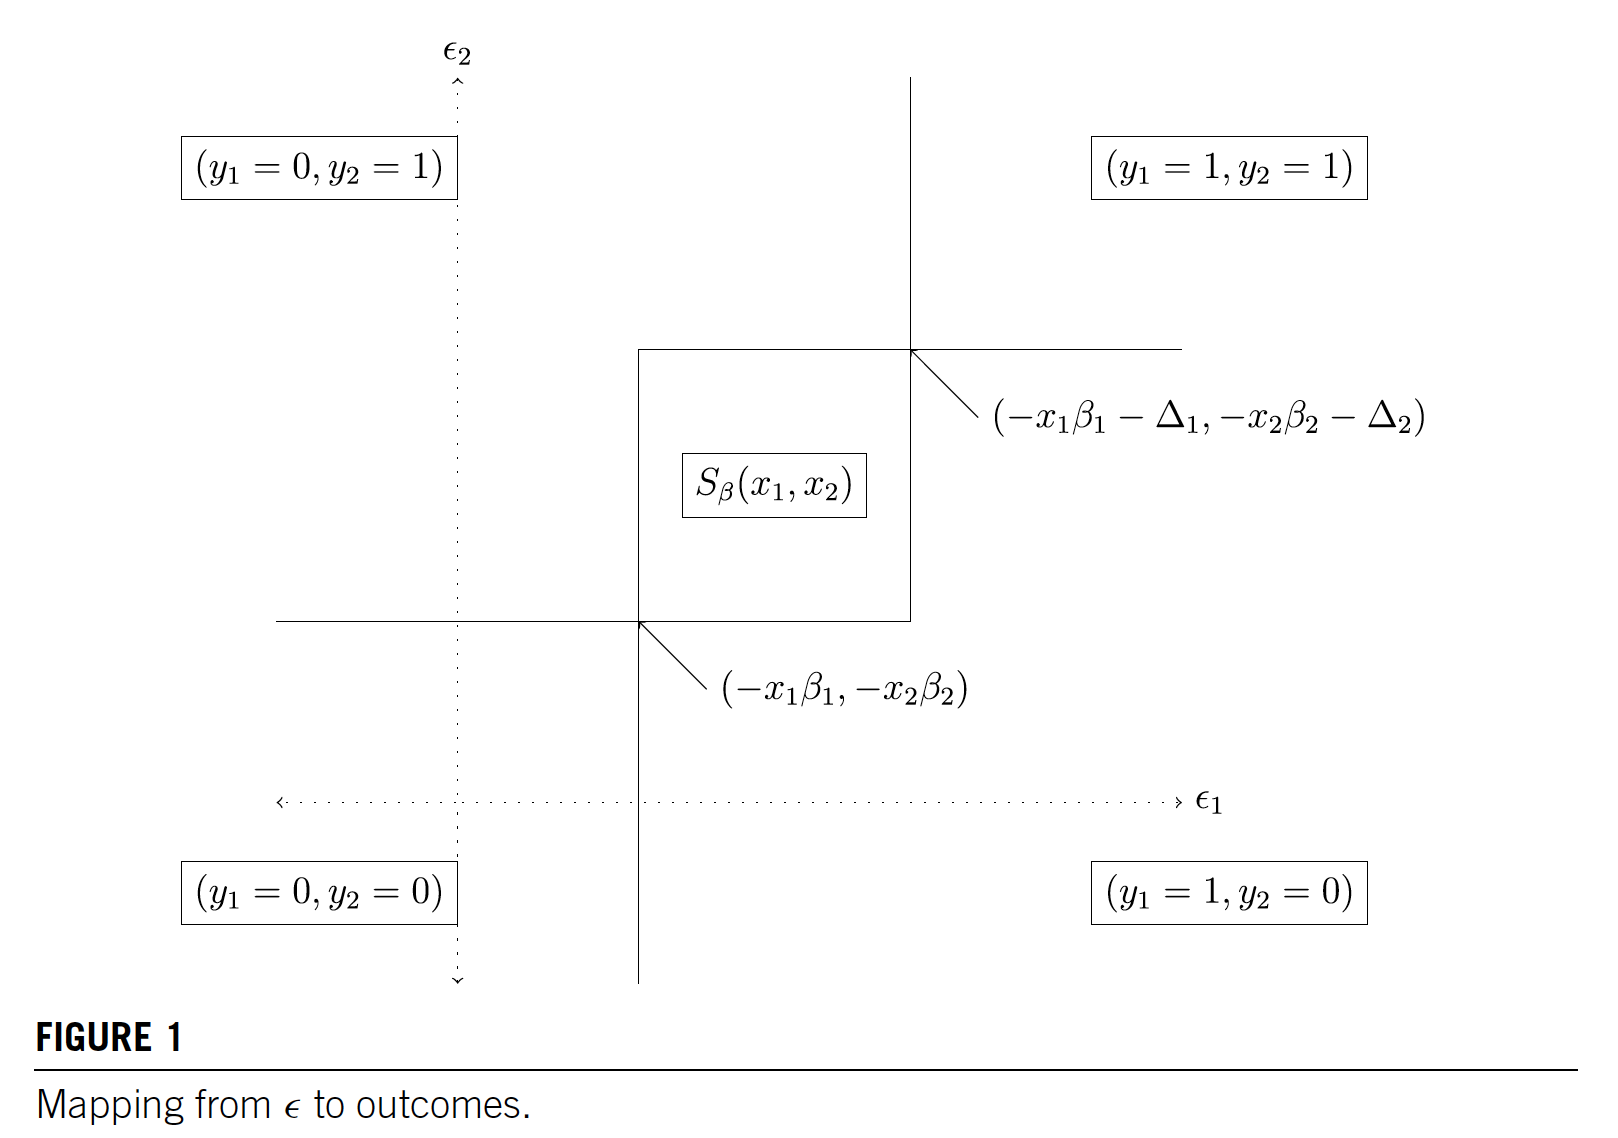
\includegraphics[width=0.7\textwidth]{multiple equil.png}
\end{figure}
\end{frame}

\begin{frame}{A Market Entry Game with Complete Information (Cont'd)}
\begin{itemize}
\item More assumptions are needed to specify the equilibrium selection rules to get a point identification of $\theta$;
\item Instead, without any further assumptions, we can still get a set of $\theta$ by using partial identification approach:
\item The inequality conditions are coming from the statistical property of the probability. We apply this inequality condition on the ones we do not have a function of $\theta$: $\textcolor{red}{P \left(d_1 = 1, d_2 =0 | x, \epsilon \in S_\beta \right) \in [0, 1]}$.
\item Thus, we find the set of $\theta$ that satisfies the inequality conditions:
    \begin{align*}
        H_L^{(1,0)}\leq P(d_1 = 1, d_2 = 0 | x) \leq H_U^{(1,0)}
    \end{align*}
    \item Where $H_L^{(1,0)} = P \left(\epsilon_1 \geq -x_1 \beta_1, \epsilon_2 \leq -x_2 \beta_2 - \Delta_2, \epsilon \notin S_\beta \right)$,
    \item $H_U^{(1,0)} = P \left(\epsilon_1 \geq -x_1 \beta_1, \epsilon_2 \leq -x_2 \beta_2 - \Delta_2\right)$.
\end{itemize}
\end{frame}

\begin{frame}{A Market Entry Game with Complete Information (Cont'd)}
\begin{itemize}
    \item Similar approach for $p_{01} = p\left(d_1 = 0, d_2 = 1 | x\right)$ to find $H_L^{(0,1)}$ and $H_U^{(0,1)}$.
    \item For $p_{00}$ and $p_{11}$, we have equality conditions, which can be written as functions of $\theta$: $H^{(0,0)} = P \left(\epsilon_1 \leq -x_1 \beta_1, \epsilon_2 \leq -x_2 \beta_2\right)$ and $H^{(1,1)} = P \left(\epsilon_1 \geq -x_1 \beta_1 - \Delta_1, \epsilon_2 \geq -x_2 \beta_2 - \Delta_2\right)$.
    \item Finally, the identified set of $\theta$ is the intersection of the sets from all conditions:
    \begin{equation*}
            \begin{aligned}
            \Theta = \{\theta: &H_L^{(1,0)}\leq P(d_1 = 1, d_2 = 0 | x) \leq H_U^{(1,0)}, \\
                            &H_L^{(0,1)}\leq P(d_1 = 0, d_2 = 1 | x) \leq H_U^{(0,1)}, \\
                            &P(d_1 = 0, d_2 = 0 |x) = H^{(0,0)}, \\
                            &P(d_1 = 1, d_2 = 1 | x) = H^{(1,1)} \}
            \end{aligned}
    \end{equation*}
\end{itemize}
\end{frame}

\begin{frame}{Other Strategic Interaction Models: Incomplete Information}
A market entry game with incomplete information:
\begin{itemize}
    \item With incomplete information, firms form beliefs about the other firm's action based on what they know:
    \item The payoffs are now functions of the actions and the beliefs of the other firm:
    \begin{align*}
        \pi_1 = d_1 \times (x_1 \beta_1 + \Delta_1 \omega_1(d_2 = 1| x) + \epsilon_1) \\
        \pi_2 = d_2 \times (x_2 \beta_2 + \Delta_2 \omega_1(d_1 = 1 | x) + \epsilon_2)
    \end{align*}
    \item Where $\omega_1(d_2 = 1| x)$ is the belief that firm 1 holds about the probability that firm 2 will enter the market.
    \item By using economic theory, one can find the upper and lower bounds of $\omega_i(d_{-i} = 1| x)$, and then find the set of $\theta$ that satisfies the moment inequalities.
\end{itemize}

\end{frame}

\begin{frame}{Other Strategic Interaction Models: Auctions}
\begin{itemize}
    \item In a typical auction model, bidder $i$ with valuation $\theta_i$ has the pay-off: $\theta_i x_i - t_i$ where:
        \begin{itemize}
        \item $t_i$ is the actual transfer he made,
        \item $x_i \in \{0, 1\}$ gives the allocation state of the object,
        \item bidder $i$ bids with $b_i$.
        \end{itemize}

    \item Haile and Tamer (2003) proposes two assumptions in auction settings:
    \begin{itemize}
    \item Bids are weakly less than corrsponding valuation: $b_i(\theta_i) \leq \theta_i$;
    \item A bidder that loses the auction has a valuation that makes it unprofitable to beat the winning bid: $\theta_i \leq b^* + \Delta$
    \item Where $b^*$ is winning bid, $\Delta \geq 0$ is the minimum bid increment.
    \end{itemize}
    \item These two assumptions generate upper and lower bounds on the distributions of valuation $\theta_i$, a partial identification approach.
\end{itemize}
\end{frame}


\begin{frame}{Revisit the Roadmap}
    \begin{itemize}
        \item Partial identification is widely used in empirical IO, especially in
        \begin{itemize}
            \item Models with measurement errors or unobserved heterogeneity,
            \item Models based on revealed preference,
            \item Strategic interaction models among multiple agents (e.g., market entry, auction),
            \item Models with multiple equilibria or incomplete information.
        \end{itemize}
    \vspace{0.5cm}
        \item Partial identification also gives challenges for estimation and inference:
        \begin{itemize}
            \item Estimation: How do we estimate a set? What is a ``good" estimate of set?
            \item Inference: How to test an hypothesis about true parameters with partial identification?
        \end{itemize}
    \end{itemize}
\end{frame}

% Section 5
\section{Estimation and Inference in Partial Identification}

\end{document} 